\documentclass[a4paper, 12pt]{article}
\usepackage[utf8]{inputenc}
\usepackage{listings}
\usepackage{graphicx}
\title{Classifying car price ranges}
\author{Sivert M. Skarning}
\date{Mai 2019}
\begin{document}
\maketitle
\clearpage

\section{Introduction}
\subsection{Problem set}
Today everything is moving online. Advertising your car by using services online is very common. So how much is your car worth? How do you categorize the price range of your car? This project focuses on how to predict the value of car, based the car features.

The dataset choosen for this project is the car evaluation data set created by Marko Bohanec. This dataset contains information about 1728 cars.

\begin{itemize}
  \item buying: vhigh, high, med, low.
  \item maint: vhigh, high, med, low.
  \item doors: 2, 3, 4, 5more.
  \item persons: 2, 4, more.
  \item lug-boot: small, med, big.
  \item safety: low, med, high.
  \item Acceptibility: unnac, acc, good, v-good
\end{itemize}

Based on maintainence costs, number of doors, how many persons that fits in the car, boot size, acceptibility and safety rating we will try to make a model that predicts the buying price of the car. The model will use 6 predictors to classify wich class the car is in. The predictors are maintainence, number of doors, number of persons that can fit in the car, luggage size, acceptibility and safety.


\subsection{Dataset}
\paragraph{Usage}
The car evaluation has been referenced in many scientifc papers. Amongst the most noteworthy are:
\begin{itemize}
\item MML Inference of Decision Graphs with Multi-way Joins and Dynamic Attributes \cite{mml-interference}
\item Stopping Criterion for Boosting-Based Data Reduction Techniques: from Binary to Multiclass Problem \cite{boosting}
\item Impact of learning set quality and size on decision tree performance \cite{learning-set}
\end{itemize}

The data set was used as an example for displaying multiattribute decition-making \cite{dataset-usage}.

\paragraph{Generation}
According to Bohanec the Car evaluation data set was created from a hierarchical decition model. This model was created for the demonstration of a decition makeing software called DEX \cite{dataset}.

\section{Classification}
\subsection{C5.0}
I decided to use C5.0 for the classification. It is free and easy use. C5.0 is an algorithm to produce decition trees for classification purposes. For configuring the data and running the algorithm I used R. In R you can use the C5.0 package to generate basic tree-models and rule-based models. In this chapter I will present my findings when using this algorithm on the car evaluation dataset. To help me get started with R and the c5.0 algorithm I used this guide.

\subsection{Findings}
When running the C5.0 algorithm on the car evalutation dateset we found that the accrucy was not very high. We got a 55 percent error rate when using all the predictors. The summary of the first run can bee seen in figure \ref{fig:tree-summary} and the decition tree generated can be seen in figure \ref{fig:decition-tree}.
  \begin{figure}[h]
    \centering 
    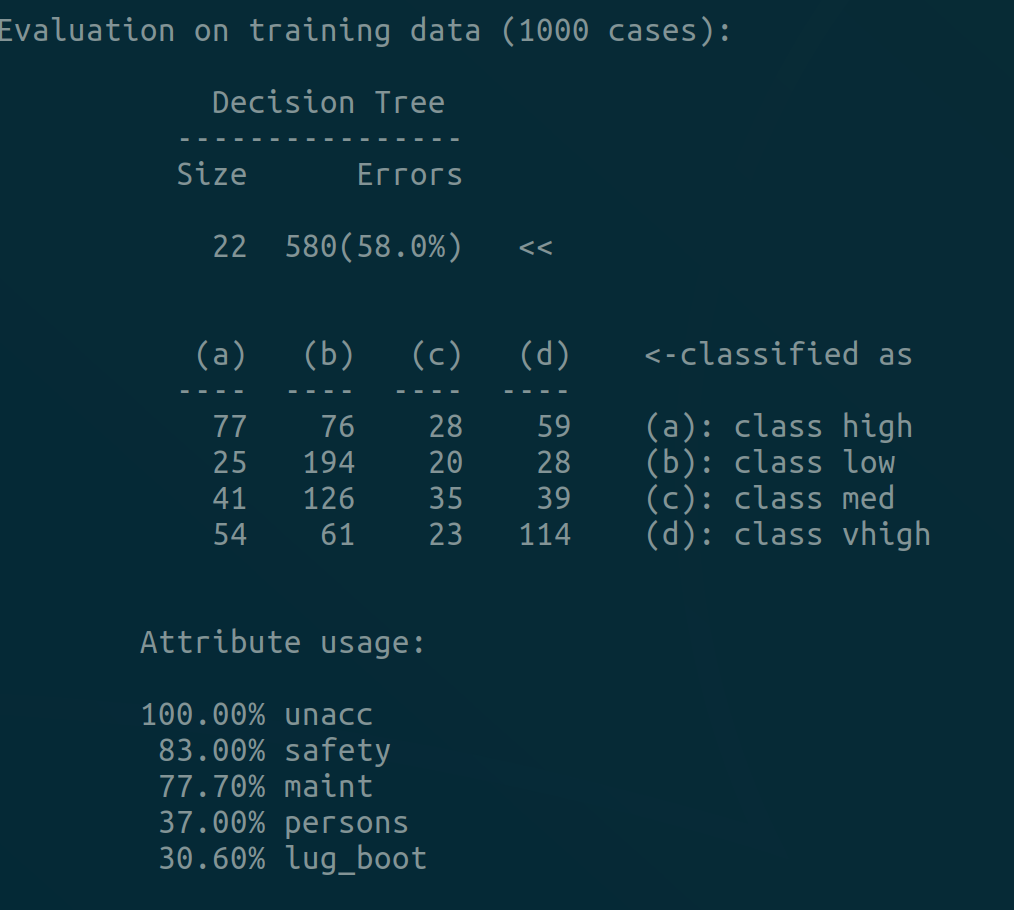
\includegraphics[width=0.6\textwidth]
    {images/summary}
    \caption{tree-summary}
    \label{fig:tree-summary}
  \end{figure}

  \begin{figure}[h]
    \centering 
    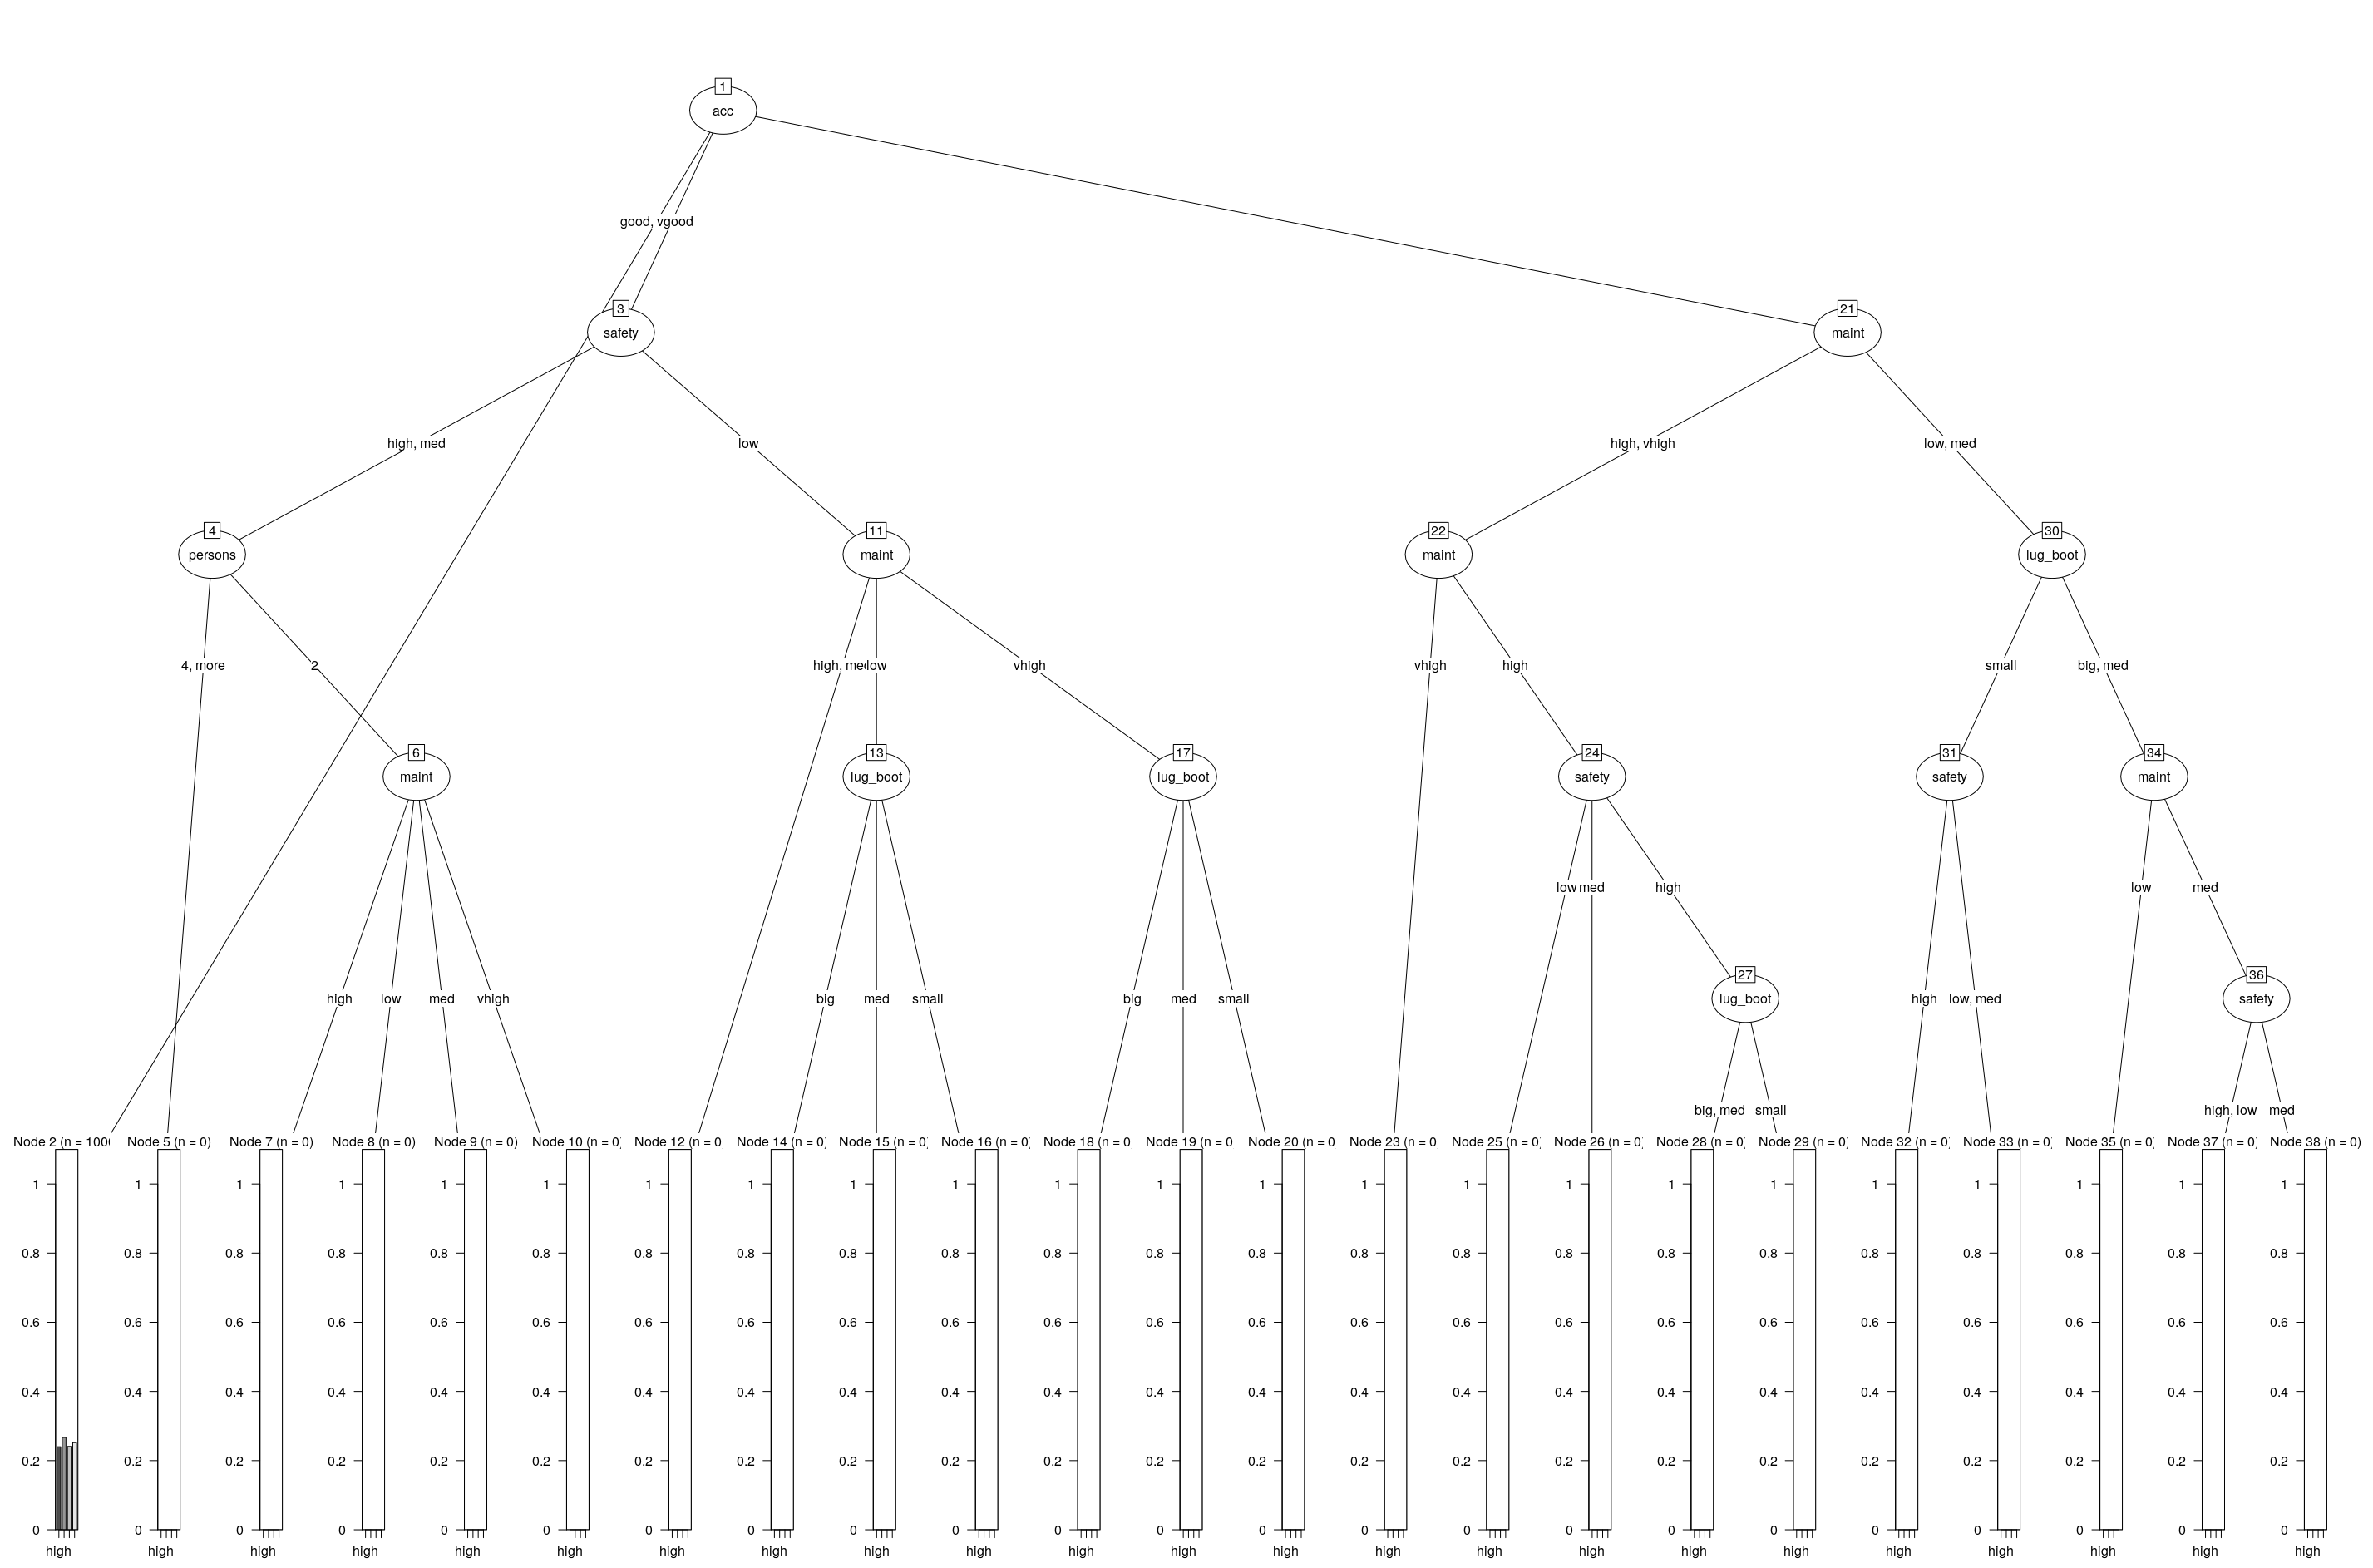
\includegraphics[width=0.6\textwidth]
    {images/tree}
    \caption{Decition-tree}
    \label{fig:decition-tree}
  \end{figure}
  \subsection{Trees and rules}
  When comparing trees in figure \ref{fig:tree-summary} and rules in figure \ref{fig:rules} we see that the error rate is similar. The tree has a slightly better error rate. This is expected because rules are a simplified tree. The rules consists of if-then rules. The rules makes it easier to read, however it might yield a slightly worse result.
  \begin{figure}[h]
    \centering 
    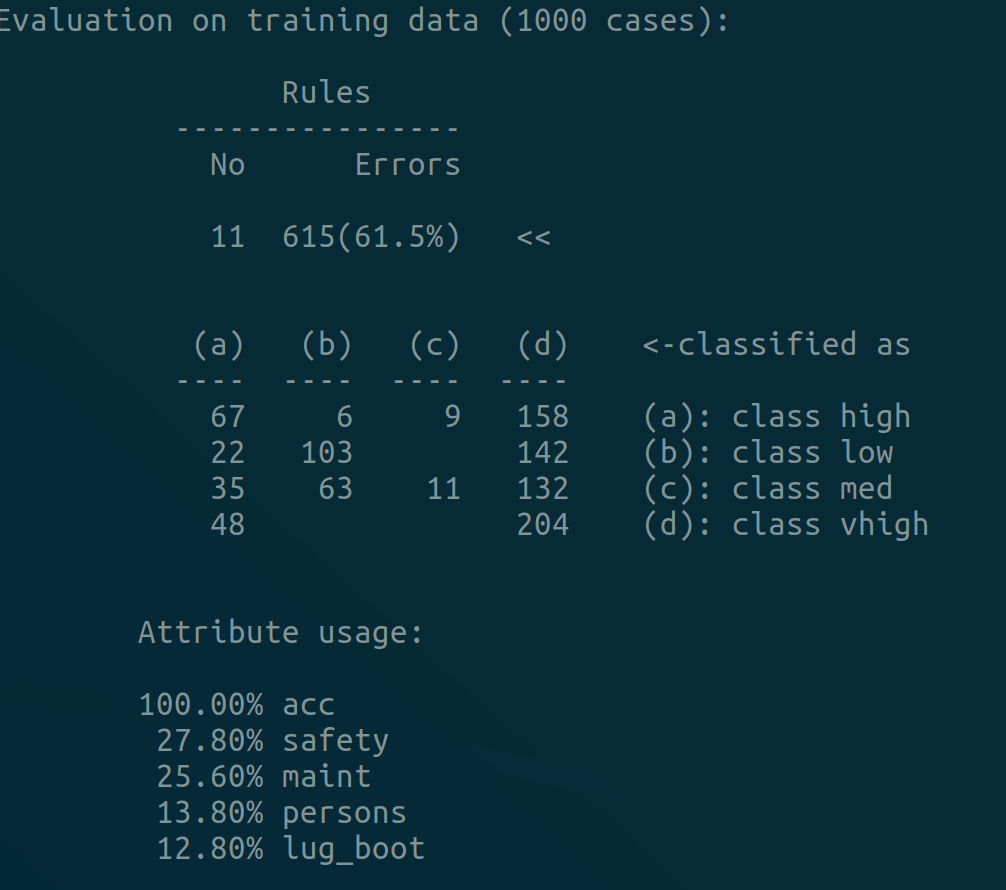
\includegraphics[width=0.6\textwidth]
    {images/summary-rules}
    \caption{Rules}
    \label{fig:rules}
  \end{figure}
  

\clearpage
\begin{thebibliography}{9}
\bibitem{mml-interference} 
peter J Tan, David L Towe, 2003
\textit{MML Inference of Decision Graphs with Multi-way Joins and Dynamic Attributes
}.

\bibitem{boosting}
  Marc Sebban, Richard Nock, Stéphane Lallich, 2002
  \textit{Stopping Criterion for Boosting-Based Data Reduction Techniques: from Binary to Multiclass Problems}.

\bibitem{learning-set}
  M. Sebban, R. Nock2, J.H. Chauchat and R. Rakotomalala
  \textit{Impact of learning set quality and size on decision tree performance}

\bibitem{dataset}
  Marko Bohanec
  \textit{http://archive.ics.uci.edu/ml/datasets/Car+Evaluation}

\bibitem{dataset-usage}
  Marko Bohanec, Vladislav Rajkovic
  \textit{Knowledge acquisition and explanation for multi-attribute decision making}

 
\end{thebibliography}
\end{document}


%%% Local Variables:
%%% mode: latex
%%% TeX-master: t
%%% End:

